\documentclass[letterpaper, 10 pt, conference]{ieeeconf}
%\documentclass[a4paper, 10pt, conference]{ieeeconf}

\overrideIEEEmargins

\usepackage[utf8]{inputenc}
\usepackage[T1]{fontenc}
\usepackage{hyperref}
\usepackage{url}
\usepackage{graphicx}
\usepackage{ngerman}

\hypersetup{hidelinks}

\title{\LARGE
\textbf{FireForceDefense} \\ Technical Report
}

\author{Cameron Barbee, Tim Hoffmann,  Christian Piffel,  Tobias Schotter,\\  Sebastian Schuscha,  Philipp Stangl,  Thomas Stangl%
}

\begin{document}

\maketitle
\thispagestyle{empty}
\pagestyle{empty}

\section{Einführung und Ziele}

Im vorliegenden Projekt soll das Tower-Defense-Spiel „FireForceDefense“ erweitert werden.
Ziel ist es, das Spiel um eine einfache Benutzerverwaltung, d.h. Registrierung und Anmeldung, zu ergänzen.
Außerdem soll eine Rangliste geschaffen werden, wofür eine Spielstand-Speicherung notwendig ist.

\section{Bausteinsicht}
Diese Sicht zeigt die statische Zerlegung des Systems in Bausteine sowie
deren Beziehungen.  %\cite{c1}

\begin{figure}[thpb]
      \centering
      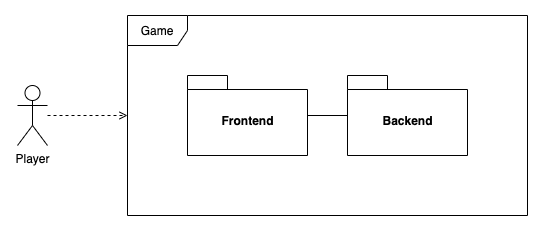
\includegraphics[scale=0.38]{images/context}
      \caption{Kontextabgrenzung}
      \label{fig:context}
\end{figure}


\subsection{Gesamtsystem}
%Whitebox-Beschreibung des Gesamtsystems,
%zusammen mit Blackbox-Beschreibungen der darin enthaltenen Bausteine.
Die Anwendung basiert auf einer Client-Server-Architektur (\ref{fig:context}).
Frontend und Backend kommunizieren über eine RESTful-API.


\subsection{Frontend}
Dieser Abschnitt beschreibt die client-seitige Frontend-Architektur.
Das Frontend wird unter Zuhilfenahme des Frameworks Vue.js realisiert.

Es ist selbst in mehrere Unter-Bausteine zerlegt:

\subsubsection{Model}

Dieser Baustein enthält die Logik für den Problembereich im Frontend.
Die eigentlichen Anzeigekomponenten besitzen Referenzen auf die Instanzen der Klassen des Model-Bereichs,
sodass Eingaben an das Model weitergegeben und dort verarbeitet werden können.
Schließlich besitzt das Model Schnittstellen, mittels denen Informationen über den aktuellen Zustand abgefragt werden können,
um basierend darauf die Anzeige anzupassen.

Im Model ist beispielsweise die Spiellogik und die Schnittstelle zum Speichern und Abrufen von Spielständen verortet.

\subsubsection{Components}

In diesem Modul sind die Vue-Komponenten gesammelt, mit denen die eigentliche Anzeige im Webbrowser realisiert wird.
Die Komponenten sind dabei hierarchisch geordnet, so besteht ein Level beispielsweise aus einer Sidebar und der LevelMap,
die LevelMap wiederum enthält einzelne Zellen und so weiter.

Die Komponenten behandeln alle Eingaben und senden bei Bedarf entsprechende Nachrichten an das Model.

\subsubsection{SCSS}

Hier werden zentral genutzte Stile im SCSS-Format abgelegt.

\subsubsection{Lang}

Dieser Baustein ist für die Internationalisierung, genauer gesagt die Übersetzung, zuständig.
Aktuell ist lediglich eine deutsche Sprachvariante hinterlegt.

\subsubsection{Levels}

Dieses Modul enthält die Level-Definitionen.
Eine Level-Definition beschreibt den initialen Aufbau des Spielfelds und die auftretenden Effekte.
Jedes Level muss anhand der jeweiligen Definition im LevelManager des Model-Bereichs registriert werden.

\subsubsection{Cells, Contents und Effects}

In diesen drei Bausteinen sind die verschiedenen, konkreten Zell-, Inhalts- bzw. Effekt-Typen samt ihren jeweiligen Eigenschaften hinterlegt.

\subsection{Backend}
Dieser Abschnitt beschreibt die server-seitige Backend-Architektur.

\subsubsection{Datenbank}

Die Speicherung der Daten erfolgt im dokumentenorientierten NoSQL-Datenbankmanagementsystem \textit{MongoDB}.  Zusätzlich wird die Bibliothek  \textit{mongoose} für das Object Data Modeling (ODM) verwendet.  \\

Grundlegend wurden die Daten in drei Collections unterteilt:
\begin{itemize}
\item
\textit{Accounts:} Hier werden die nötigen Informationen eines Benutzers gespeichert, um
eine Login- und Registrierungsfunktion zu gewährleisten. Das wäre einerseits ein
einzigartiger Benutzername, eine E-Mailadresse, ein verschlüsseltes Passwort, sowie
ein Datum, welches den Registrierungszeitpunkt festhält.
\item
\textit{Refreshtokens:} In dieser Dokumentensammlung werden alle nötigen Informationen für
das Session-Handling gespeichert. Das wäre einerseits die von MongoDB automatisch
erstellte ID der einzelnen Benutzer, um jedem Benutzer seinen entsprechenden Token
zuweisen zu können. Dazu wird der entsprechende Token gespeichert, sowie ein Verfallsdatum
des Tokens, ein Erstellungsdatum des Dokumentes und abschließend ein Wert, welcher die
IP des Erstellers festhält.
\item
\textit{Scores:} Diese Sammlung an Dokumenten speichert grundlegend alle relevanten Aspekte des
Spielstandes. Einerseits den Benutzernamen, das Level, die erreichten Sterne, das
übriggebliebene Geld, sowie die verwendete Zeit und die Anzahl an verbrannten Zellen.
Anhand dieser Informationen wird die Reihenfolge der Rangliste berechnet.
\end{itemize}

\subsubsection{Laufzeitumgebung}

JavaScript-basierte Plattform Node.js mit dem serverseitigen Webframework ExpressJS.

\section{Verteilungssicht}
Das Spiel wird in einem Docker Container bei dem Cloud-Anbieter \textit{Amazon Web Services} bereitgestellt. \\

Dieser Abschnitt beschreibt:
\begin{itemize}
\item
  die Verteilung des Gesamtsystems,
\item
  wichtige Begründungen für diese Verteilungsstruktur,
\item
  Qualitäts- und/oder Leistungsmerkmale dieser Infrastruktur,
\item
  Zuordnung von Softwareartefakten zu Bestandteilen der Infrastruktur
\end{itemize}

\section{Querschnittliche Konzepte}

Dieser Abschnitt beschreibt übergreifende, prinzipielle Regelungen und
Lösungsansätze, die an mehreren Stellen relevant sind.

\subsection{\texorpdfstring{\emph{\textless Konzept
1\textgreater{}}}{\textless Konzept 1\textgreater{}}}

\emph{\textless Erklärung\textgreater{}}

\subsection{\texorpdfstring{\emph{\textless Konzept
2\textgreater{}}}{\textless Konzept 2\textgreater{}}}

\emph{\textless Erklärung\textgreater{}}

\begin{thebibliography}{99}
% APA-Citation https://www.scribbr.de/category/apa-standard/

% Book
\bibitem{c1} Schmidt, B. (2020). Richtig zitieren: Eine Anleitung für Studierende (2. Aufl.). Springer.

% Website
\bibitem{c2} Erichsen, C. (2020, 17. Juli). Inklusion im Internet: So werden Social-Media-Inhalte barrierefrei. \url{t3n. https://t3n.de/magazin/inklusion-im-internet-so-werden-249553/}

\end{thebibliography}


\addtolength{\textheight}{-12cm}

\end{document}
